

	\section{Материалы}
	
	
	\begin{figure}
	    \centering
	    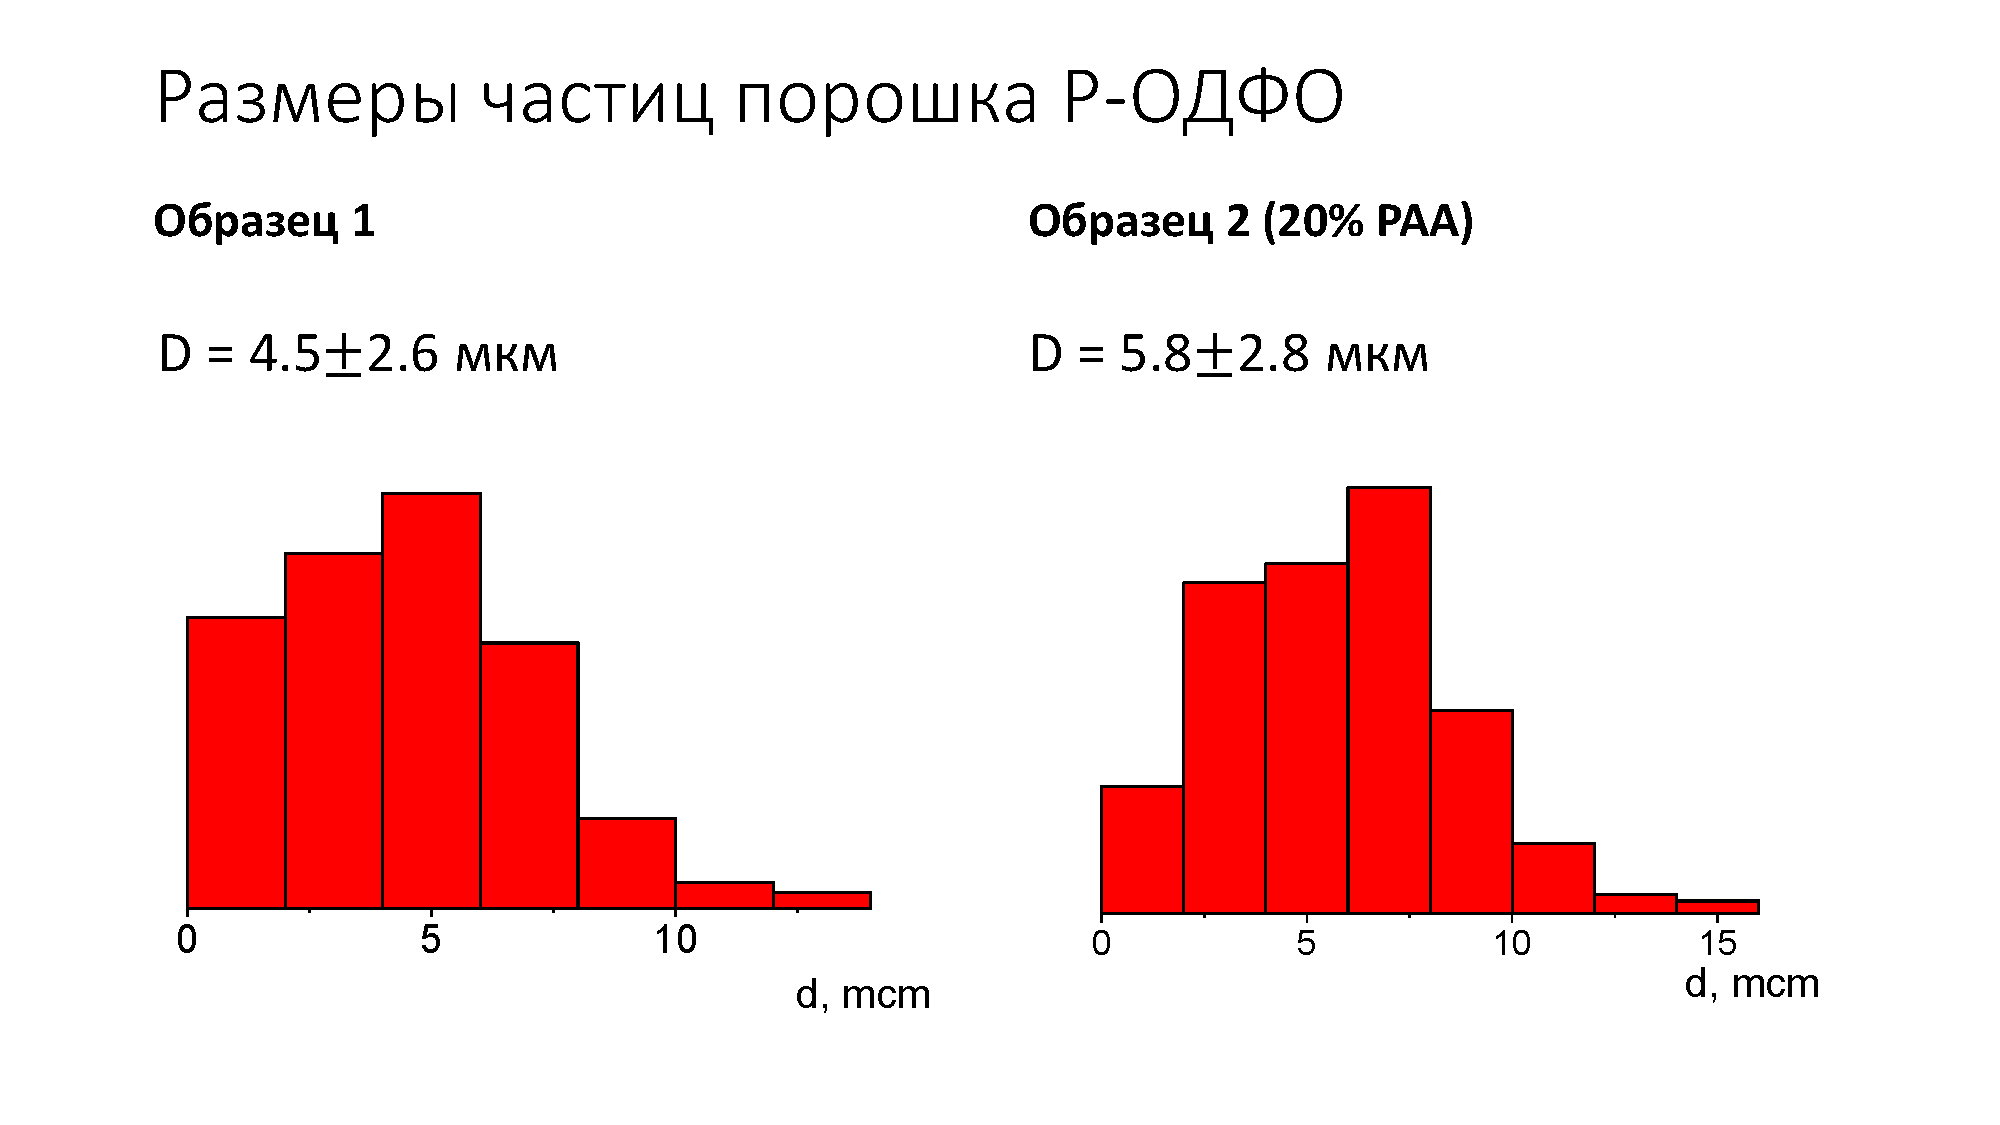
\includegraphics[width=\linewidth]{fig/particles}
	    \caption{Caption}
	    \label{fig:my_label}
	\end{figure}
	
	\section{Схема эксперимента}
	
	\section{Получение и первичная обработка данных}
	
	\section{Вычитание фона, аппроксимация пиков}
	
	\begin{lstlisting}[language=Python, caption=Python example]
import numpy as np
 
def incmatrix(genl1,genl2):
    m = len(genl1)
    n = len(genl2)
    M = None #to become the incidence matrix
    VT = np.zeros((n*m,1), int)  #dummy variable
 
    #compute the bitwise xor matrix
    M1 = bitxormatrix(genl1)
    M2 = np.triu(bitxormatrix(genl2),1) 
 
    for i in range(m-1):
        for j in range(i+1, m):
            [r,c] = np.where(M2 == M1[i,j])
            for k in range(len(r)):
                VT[(i)*n + r[k]] = 1;
                VT[(i)*n + c[k]] = 1;
                VT[(j)*n + r[k]] = 1;
                VT[(j)*n + c[k]] = 1;
 
                if M is None:
                    M = np.copy(VT)
                else:
                    M = np.concatenate((M, VT), 1)
 
                VT = np.zeros((n*m,1), int)
 
    return M
\end{lstlisting}
	
	\section{Карты кристалличности}
	
	\section{Параметры решетки, расчеты}
	

	
	\paragraph{интегрирование распознавание пиков}
	че получили:
		\begin{figure}
    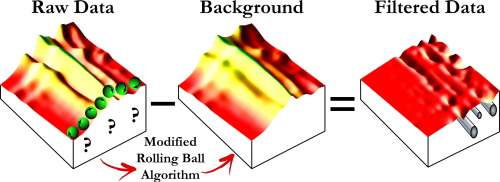
\includegraphics[width=\textwidth]{fig/rolling-ball.jpg}
    \caption{Принцип работы алгоритма}
    \label{fig:rolling-ball}
\end{figure}
	
	\paragraph{Rolling-ball}
	погрешности, чем хорошо, почему он, какие еще бывают
	
	А код - в приложении!
	
	\begin{figure}
    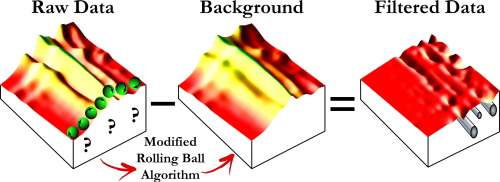
\includegraphics[width=\textwidth]{fig/rolling-ball.jpg}
    \caption{Принцип работы алгоритма}
    \label{fig:rolling-ball}
\end{figure}

    \paragraph{фиттинг}

\begin{figure}
    \centering
    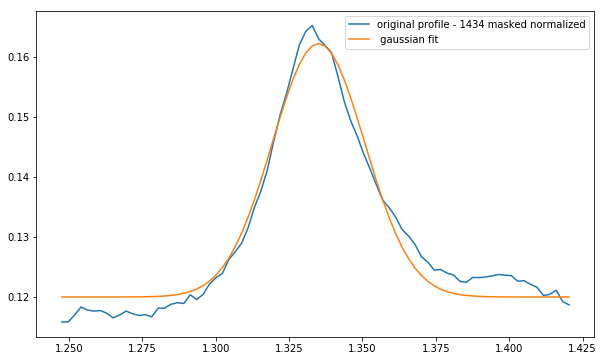
\includegraphics[width=\linewidth]{fig/gauss-fit.png}
    \caption{Аппроксимация формы пика по разным моделям}
    \label{fig:my_label}
\end{figure}
	
	\paragraph{Карты кристалличности}
	
	\begin{figure}[ht]\center
\begin{tabular}{cc}
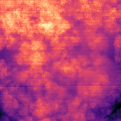
\includegraphics[width=0.5\linewidth]{fig/map-1.png}
&
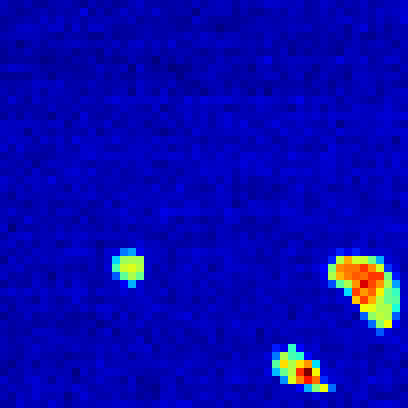
\includegraphics[width=0.5\linewidth]{fig/map-2.png}
\end{tabular}
\caption{Карты кристалличности}
\end{figure}
	
	

	
	
	
	Свойства и результаты прочих исследований:
	[Vaganov corrected]